%!TEX root = ../../thesis.tex
\section{Node Graph}
\label{impl-node-graph}

\begin{figure}[htb]
  \centerline{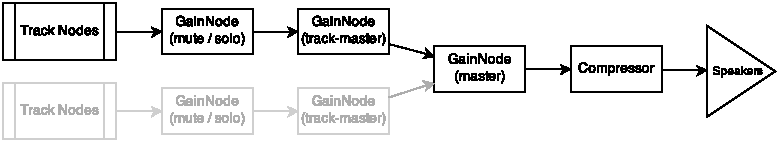
\includegraphics[width=\linewidth]{images/Node_Graph.pdf}}
  \caption[The editor's audio node graph]{The editor's audio node graph}
  \label{fig:nodegraph}
\end{figure}

\reffigure{fig:nodegraph} shows the editor's basic audio graph setup. Each track is wired in the same way. All individual audio nodes of a track (e.g. \code{BufferSourceNodes} in case of a recording track) are connected to their `mute / solo' \code{GainNode}. A \code{GainNode} is an audio node that controls the gain of all the nodes that are connected to it. The `mute / solo' \code{GainNode} controls a track's gain, when its `mute' or `solo' attribute changes. A muted track will have a gain value of \code{0} when its \code{mute} attribute is \code{true} and it will have a gain value of \code{1} if either its \code{mute} attribute or its \code{solo} attribute is \code{true}. All other tracks will have a \code{false solo} attribute if one of the tracks has a \code{true solo} attribute and their \code{gain} value will be \code{0}.

The `track-master' \code{GainNode} controls the overall gain value of the track, which is represented by a track's \code{gain} attribute. This attribute is synchronized and persisted across all clients. By separating the `track-master' from the `mute / solo' node, the editor has fine-grained control about the individual gain settings of the tracks and users can individualize their local track setup without interfering with other users' setups (e.g., if User A mutes track B and user C is currently working on track B's details, user C's track is not muted and he is still able to work on it).

Each track's `track-master' \code{GainNode} is connected to the editor's `master' \code{GainNode}. It controls the overall gain level. Its value is also not synchronized so that each user has full control over the playback's volume.

Before the editor's signal goes to the speakers, it is passed through a `compressor'. This node's purpose is to create a more homogeneous sound signal and to prevent the signal from being clipped because it is too loud. The Web Audio API already provides a node for this purpose, the \code{DynamicsCompressor Node}\footnote{\url{http://webaudio.github.io/web-audio-api/\#idl-def-DynamicsCompressorNode}, last checked on 21/03/2014}. It is also this node, which is used to record the arrangement (see \refchapter{impl-arrangement-recording}).

The node setup of all the different types of nodes is explained in detail in their individual implementation chapters. The `last' node in their setup always connects to the track's `mute / solo' node to pass its signal into the editor's node graph.